%% LyX 2.4.3 created this file.  For more info, see https://www.lyx.org/.
%% Do not edit unless you really know what you are doing.
\documentclass[aspectratio=169]{beamer}
\usepackage{mathpazo}
\usepackage{booktabs}
\usepackage[latin9]{inputenc}
\setcounter{secnumdepth}{3}
\setcounter{tocdepth}{3}
\usepackage{array}
\usepackage{multirow}
\usepackage{amstext}
\usepackage{amssymb}
\usepackage{graphicx}
\usepackage{tikz}
\usepackage{appendixnumberbeamer}
\usetikzlibrary{patterns}
\usepackage{standalone}
\ifx\hypersetup\undefined
  \AtBeginDocument{%
    \hypersetup{bookmarks=false,
 breaklinks=false,pdfborder={0 0 1},backref=section,colorlinks=false}
  }
\else
  \hypersetup{bookmarks=false,
 breaklinks=false,pdfborder={0 0 1},backref=section,colorlinks=false}
\fi

\makeatletter

%%%%%%%%%%%%%%%%%%%%%%%%%%%%%% LyX specific LaTeX commands.
%% Because html converters don't know tabularnewline
\providecommand{\tabularnewline}{\\}

%%%%%%%%%%%%%%%%%%%%%%%%%%%%%% Textclass specific LaTeX commands.
% this default might be overridden by plain title style
\newcommand\makebeamertitle{\frame{\maketitle}}%
% (ERT) argument for the TOC
\AtBeginDocument{%
  \let\origtableofcontents=\tableofcontents
  \def\tableofcontents{\@ifnextchar[{\origtableofcontents}{\gobbletableofcontents}}
  \def\gobbletableofcontents#1{\origtableofcontents}
}

%%%%%%%%%%%%%%%%%%%%%%%%%%%%%% User specified LaTeX commands.
%\newtheorem{theorem}{Theorem}
%\newtheorem{corollary}[theorem]{Corollary}
%\newtheorem{definition}[theorem]{Definition}
%\newtheorem{example}[theorem]{Example}
%\newtheorem{lemma}[theorem]{Lemma}
%\newtheorem{problem}[theorem]{Problem}
%\newtheorem{solution}[theorem]{Solution}


%%%%%%%%%%%%%%%%%%%%%%%%%%%%%%%%%%%%%%%%%%%%%%%%%%%%%%%%%%%%%%%%%%%%%%%%%%%%%%%%%%%%%%%%%%%%%%%%%%%%%%%%%%%%%%%%%%%%%%%%%%%%%%%%%%%%%%%%%%%%%%%%%%%%%%%%%%%%%%%%%%%%%%%%%%%%%%%%%%%%%%%%%%%%%%%%%%%%%%%%%%%%%%%%%%%%%%%%%%%%%%%%%%%%%%%%%%%%%%%%%%%%%%%%%%%%
\usepackage{graphicx}
\usepackage{amsfonts}
\usepackage{multimedia}
\usepackage{pstricks}
%\usepackage{pst-plot}
\usepackage{xcolor}
\beamertemplatenavigationsymbolsempty
\date{} 
\setbeamertemplate{footline}[frame number]

\setcounter{MaxMatrixCols}{10}
%TCIDATA{OutputFilter=LATEX.DLL}
%TCIDATA{Version=5.50.0.2953}
%TCIDATA{<META NAME="SaveForMode" CONTENT="2">}
%TCIDATA{BibliographyScheme=Manual}
%TCIDATA{Created=Friday, October 09, 2009 16:36:30}
%TCIDATA{LastRevised=Monday, April 01, 2013 11:48:45}
%TCIDATA{<META NAME="GraphicsSave" CONTENT="32">}
%TCIDATA{<META NAME="DocumentShell" CONTENT="Other Documents\SW\Slides - Beamer">}
%TCIDATA{CSTFile=beamer.cst}

\newtheorem{acknowledgement}[theorem]{Acknowledgement}\newtheorem{algorithm}[theorem]{Algorithm}\newtheorem{axiom}[theorem]{Axiom}\newtheorem{case}[theorem]{Case}\newtheorem{claim}[theorem]{Claim}\newtheorem{conclusion}[theorem]{Conclusion}\newtheorem{condition}[theorem]{Condition}\newtheorem{conjecture}[theorem]{Conjecture}\newtheorem{criterion}[theorem]{Criterion}\newtheorem{exercise}[theorem]{Exercise}\newtheorem{notation}[theorem]{Notation}\newtheorem{proposition}[theorem]{Proposition}\newtheorem{remark}[theorem]{Remark}\newtheorem{summary}[theorem]{Summary}\newtheorem{prediction}{Prediction}\setbeamertemplate{itemize items}[circle]
\setbeamercolor{itemize item}{fg= black}
\setbeamercolor{itemize subitem}{fg=black}
\setbeamercolor{itemize subsubitem}{fg= black}
\setbeamercolor{frametitle}{fg=purple}
\setbeamercolor{title}{fg=black}
\setbeamercolor{caption name}{fg=black}


%
\usefonttheme{serif}
\setbeamersize{text margin left=5pt,text margin right=5pt}
%%\usetheme{Singapore}
\usetheme{default}
%%\input{tcilatex}
%\useoutertheme{miniframes}
%\hypersetup{colorlinks=true,linkcolor=white}
%%\setbeamertemplate{footline}[frame number]
%\beamertemplatenavigationsymbolsempty
%%\setbeamertemplate{footline}{\hspace*{.5cm}\scriptsize{\insertauthor\hspace*{40pt}\insertframenumber}}

%\begin{document}

\makeatother

\begin{document}
\title{{\Large\textrm{\textsc{\textcolor{violet}{AI and Human Capital Accumulation: \\
Aggregate and Distributional Implications}}}}{\LARGE\textrm{\textcolor{violet}{\medskip{}
}}}}
\author{{\large$\begin{array}{cccc}
\text{Yang K. Lu} &  &  & \text{Eunseong Ma}\\
\text{HKUST} &  &  & \text{Yonsei}
\end{array}$}~\\
\vspace{0.6cm}
~\\
{\large\color{blue}EEA \& EESM}}
\date{{\normalsize\textrm{Aug 17, 2026}}}

\makebeamertitle
\section{Introduction}

\begin{frame}{Motivation}

\begin{itemize}
\item AI's effects on labor markets are both profound and uneven
\begin{itemize}
  \item complements high-skill, substitutes middle-skill, augments lower-skill
  \item raises entry barrier for high-skill jobs
  \item[]
  {\small\textit{\textcolor{gray}{(Revelio Labs, 2025; Souza, 2025;
  Asam and Heller, 2025)}}}.
\end{itemize}
\end{itemize}
\medskip{}

\begin{itemize}
\item Workers can respond by re-optimizing \textcolor{blue}{human
capital investments.}
\begin{itemize}
\item Confidence in traditional higher education is eroding 
\item Demand for AI reskilling is surging 
\item[] {\small\textit{\textcolor{gray}{(Public
Agenda, 2022; Oliver Wyman Forum, 2024)}}}{\small\par}
\end{itemize}
\item \textit{\textcolor{brown}{Yet most studies abstract from these endogenous
human-capital responses.}}
\end{itemize}
\medskip{}

\begin{itemize}
\item This paper addresses this gap by examining 
\begin{itemize}
\item \textcolor{red}{how AI-driven changes affect human capital investment,}
\item \textcolor{red}{how human-capital adjustments reshape AI's aggregate
and distributional outcomes.}
\end{itemize}
\end{itemize}
\end{frame}

\begin{frame}{What We Do}

\begin{itemize}
\item We construct a model with human capital investment and a sectoral
structure.

\medskip{}

\item \textbf{Market Incompleteness}
\begin{itemize}
\item Households differ in assets, human capital, and idiosyncratic labor
productivity.
\item They make an indivisible labor-supply choice and a standard savings
decision.
\end{itemize}
\medskip{}

\item \textbf{\textcolor{red}{Human Capital Investment}}
\begin{itemize}
\item part-time learning vs. full-time learning
\item higher-HC sector: higher wages but more exposed to idiosyncratic productivity shock
\end{itemize}
\medskip{}

\item \textbf{\textcolor{brown}{Key Channel:}}\textcolor{brown}{{} }\textbf{\textcolor{brown}{HC investment interacts with labor supply and saving decisions.}}
\end{itemize}
\end{frame}

\begin{frame}{What We Find}

\medskip{}

\begin{itemize}
\item \textbf{We assume that AI adoption is fully anticipated}
\begin{enumerate}
\item \textbf{\textcolor{blue}{Baseline:}} AI reduces middle-level skill premium, increases high-level skill premium
\item \textbf{\textcolor{brown}{AI+:}}\textcolor{brown}{{} }AI raises the HC threshold for high-sector entry
\end{enumerate}

\medskip{}


  \item \textbf{Analytical Results from a two-period model}
  \smallskip{}
  \begin{itemize}
    \item \textbf{Heterogeneous Effects of HC investment on saving:}
  \item[] \textcolor{red}{crowds out} saving for \textcolor{red}{low-income} HHs but \textcolor{blue}{crowds in} saving for \textcolor{blue}{high-income} HHs.
  \smallskip{}
  \item \textbf{Heterogeneous Effects of AI on HC investment:}
  \item[] \textcolor{red}{reduces} HC investment for \textcolor{red}{low-HC} HHs but \textcolor{blue}{increases} it for \textcolor{blue}{high-HC} HHs.
  \end{itemize}

\medskip{}
\item \textbf{Quantitative Results from a calibrated dynamic model}

\begin{itemize}
\item \textbf{Voluntary Job Polarization} 
\item Income and earnings inequality rises due to the polarization.
\item Wealth inequality changes \textcolor{blue}{little in the baseline} but \textcolor{brown}{rises in the AI+ experiment}.
\end{itemize}

\end{itemize}
\end{frame}



\begin{frame}{Related Literature}

\begin{itemize}
\item \textbf{\textcolor{black}{Technological advancements on job polarization}}
\begin{itemize}
\item \textit{\textcolor{gray}{Goos and Manning (2007), Autor and Dorn (2013),
Goos et al. (2014), Acemoglu and Restrepo (2020)}}
\end{itemize}
\smallskip{}

\item \textbf{\textcolor{black}{Automation increases human capital investment:}}
\begin{itemize}
\item \textit{\textcolor{gray}{Atkin (2016), Beaudry et al. (2016), Dauth
et al. (2021), Di Giacomo and Lerch (2023)}}
\end{itemize}
\smallskip{}

\item \textbf{\textcolor{black}{Automation exacerbates wealth inequality}}
\begin{itemize}
\item \textit{\textcolor{gray}{Sachs and Kotlikoff (2012), Prettner and
Strulik (2020)}}
\end{itemize}
\end{itemize}
\smallskip{}

\begin{itemize}
\item \textbf{\textcolor{purple}{We analyze effects of
AI on both aggregate and distributional outcomes, highlighting the roles of human capital adjustment.}}
\end{itemize}
\end{frame}


\section{Model}
\begin{frame}{~}

\begin{center}
{\huge\textbf{Model Environment}}{\huge\par}
\par\end{center}

\end{frame}

\begin{frame}{Households{\small\textbf{\textit{\textcolor{brown}{~~Heterogeneity}}}}}

\begin{itemize}
\item \textcolor{blue}{Idiosyncratic shocks:} Households face idiosyncratic
labor-productivity and learning-ability shocks, $z$ and $y$, which
follow AR(1) process in logs: 
\end{itemize}
\medskip{}

\begin{center}
$\log z'=\rho_{z}\log z+\varepsilon_{z},\,\,\,\,\varepsilon_{z}\stackrel{iid}{\sim}\mathcal{N}(0,{\sigma_{z}}^{2})$.
\par\end{center}

\medskip{}

\begin{center}
$\log y'=\rho_{y}\log y+\varepsilon_{y},\,\,\,\,\varepsilon_{y}\stackrel{iid}{\sim}\mathcal{N}(0,{\sigma_{y}}^{2})$.
\par\end{center}
\begin{itemize}
\item \textcolor{blue}{Incomplete asset market:} Households cannot issue
any assets contingent on their future idiosyncratic risks.
\end{itemize}
\end{frame}

\begin{frame}{Households{\small\textbf{\textit{\textcolor{brown}{~~Human capital}}}}}

\begin{itemize}
\item Human capital investment can take three levels of effort: $\{0,e_{L},e_{H}\}$. 
\item A non-working HH is free to choose any of the effort levels but a
working HH cannot devote $e_{H}$: 
\end{itemize}
\begin{equation}
e_{t}\in\left\{ \begin{array}{cl}
\{0,e_{L}\} & \text{ if }n>0\\
\{0,e_{L},e_{H}\} & \text{ if }n=0
\end{array}\right.\label{eq:x-1}
\end{equation}

\medskip{}

\begin{itemize}
\item Its contribution to next-period human capital is subject to the productivity
shock: 
\begin{equation}
h_{t+1}=y_{t}e_{t}+(1-\delta)h_{t}
\end{equation}
\item Sectoral productivity for effective labor units 
\begin{equation}
x(h)=\left\{ \begin{array}{cl}
1-\lambda & \text{low sector if }h<h_{M}\\
1 & \text{middle sector if }h_{M}\leq h<h_{H}\\
1+\lambda & \text{high sector if }h\geq h_{H}
\end{array}\right.\label{eq:x}
\end{equation}
\end{itemize}
\end{frame}

\begin{frame}{Households{\small\textbf{\textit{\textcolor{brown}{~~Problem}}}} }

\begin{itemize}
\item Given $z_t$ and $y_t$, a household maximizes her expected lifetime utility by choosing consumption, saving, labor supply, and human capital investment.

\medskip{}

\begin{equation}
\max_{\left\{ c_{t},a_{t+1},n_{t},e_{t}\right\} _{t=0}^{\infty}}E_{0}\left[\sum\limits_{t=0}^{\infty}\beta^{t}(\ln c_{t}-\chi_{n}n_{t}-\chi_{e}e_{t})\right]\text{ s.t.}
\end{equation}
\textcolor{black}{
\begin{align}
c_{t}+a_{t+1} & =w_{t}z_{t}x(h_{t})n_{t}+(1+r_{t})a_{t}\\
h_{t+1}&=y_{t}e_{t}+(1-\delta)h_{t}\\
a_{t+1}&\ge0.
\end{align}
}

\item Labor supply is indivisible: $n_{t}\in\{0,\overline{n}\}$.
\end{itemize}
\end{frame}

\begin{frame}{Production technology}

\begin{itemize}
\item Produce output according to Cobb-Douglass production function: 

\begin{equation}
F(K,L)=K^{1-\alpha}L^{\alpha},
\end{equation}
\begin{equation}
K={\textstyle \int a_{i}di,\quad L={\textstyle \int n_{i}z_{i}x(h_{i})di}}
\end{equation}
\begin{equation}
    w = F_L(K,L),\quad r =F_K(K,L).
\end{equation}

\end{itemize}
\end{frame}

\begin{frame}{AI Effects}

\begin{itemize}
\item \textbf{Baseline:} AI changes skill premium through $\gamma$ {\small\textit{\textcolor{gray}{(Autor
and Dorn, 2013; Goos et al.,20145)}}}{\small\par}

\begin{equation}
x(h)=\left\{ \begin{array}{cl}
1-\lambda+\gamma\lambda & \text{low sector if }h<h_{M}\\
1 & \text{middle sector if }h_{M}\leq h<h_{H}\\
1+\lambda+\gamma\lambda & \text{high sector if }h\geq h_{H}
\end{array}\right.\label{eq:xAI-1}
\end{equation}

\medskip{}

\item \textbf{AI+:} AI raises the bar for high-sector entry: $h_H'>h_H$ {\small\textit{\textcolor{gray}{(Bloomberg,
2025)}}}{\small\par}

\begin{equation}
x^{AI+}(h)=\left\{ \begin{array}{cl}
1-\lambda+\gamma\lambda & \text{low sector if }h<h_{M}\\
1 & \text{middle sector if }h_{M}\leq h<h'_{H}\\
1+\lambda+\gamma\lambda & \text{high sector if }h\geq h'_{H}
\end{array}\right.\label{eq:xAI-1-1}
\end{equation}

\end{itemize}
\end{frame}


\section{Two-period Model}
\begin{frame}{~}

\begin{center}
{\huge\textbf{Household Decisions in Two-Period Model}}{\huge\par}
\par\end{center}

\end{frame}

\begin{frame}{}
  \begin{itemize}
      \item Period 2: work $n=1$ iff $z>\overline{z}(h,a)$ (normalize $\overline{n}=1$)
      \medskip
      \item Period 1: labor supply and HC investment $\{n,e\}$ 
      \begin{figure}
        \centering
        \scalebox{0.9}{\input{../figure_204040calib/Figure1}}
        \par
      \end{figure}
  \end{itemize}
\end{frame}



\begin{frame}{Effect of part-time learning on saving $a'$}
  Normalize $z=1$ and $\ln z' \sim \mathcal{N}(0,\sigma_z^2)$
  \begin{equation*}\label{eq:savingprob}
  \max_{a'} : \ln(c) + \beta \mathbb{E}_{z'}[\ln(c')],
  \end{equation*}
  subject to:
  \begin{equation}
  c + a' = a + x , \quad c' = a' + txz'
  \end{equation}
  The second-order approximate solution to the FOC is:
  \begin{equation}
  a'^*(x,a;t) = \underbrace{\frac{\beta(a+x) - tx\mu}{1+\beta}}_{\text{CE}} + \underbrace{\frac{t^2x^2\Sigma}{\beta(a+x + tx\mu)}}_{\text{Precautionary}}
  \end{equation}
  where $\mu\equiv \mathbb{E}[z']$ and $\Sigma \equiv\operatorname{Var}(z')$
  
  
\end{frame}
  
\begin{frame}{Effect of part-time learning on saving $a'$}
  Compare optimal $a'$ between $e=e_L$ $(t>1)$ and $e=0$ $(t=1)$
  \begin{equation} \label{eq:dadt_integral}
      \Delta_{\text{part-time}}(x,a;t) = a'^*(x,a;t) - a'^*(x,a;1) = \int_1^t \frac{\partial a'^*}{\partial u}(x,a;u) du,
  \end{equation}
  Part-time learning \textcolor{red}{\textbf{crowds out}} saving for \textcolor{red}{\textbf{low-income}} households and \textcolor{blue}{\textbf{crowds in}} saving for \textcolor{blue}{\textbf{high-income}} households.
  \begin{proposition}\label{prop:dadt}
      If $\frac{\Sigma}{\mu}>\sigma^*(t)$, $\Delta_{\text{part-time}}(x,a;t)<0$ for $x<x^\ast(a,t)$, and $\Delta_{\text{part-time}}(x,a;t)>0$ for $x>x^\ast(a,t)$.
  \end{proposition}
  
 \end{frame}

 \begin{frame}{Effect of full-time training on saving $a'$}
  \begin{itemize}
      \item Full-time training requires $n=0$.
      \item Household forgoes period-1 labor income.
  \end{itemize}
  \begin{align}
  \max_{a'} &: \ln(c) + \beta \mathbb{E}_{z'}[\ln(c')],\notag\\
  e=e_H&: \quad c + a' = a, \quad c' = a' + txz'\\
  e=0&: \quad c + a' = a + x, \quad c' = a' + xz'
  \end{align}
  \end{frame}
  
  \begin{frame}{Effect of full-time training on saving $a'$}
  Compare optimal $a'$ between $e=e_H$ $(t>1,n=0)$ and $e=0$ $(t=1)$
  \begin{align}
      \Delta_{\text{full-time}}(x,a;t) &=\Delta_{\text{part-time}}(x,a;t) + \Delta_H(x,a;t) \notag \\
      \text{where } \Delta_H(x,a;t) &\equiv x \Bigg[ -\frac{\beta}{1+\beta} + \frac{\Sigma}{\beta} \frac{t^2 x^2}{(a + x + t x \mu)(a + t x \mu)} \Bigg]
  \end{align}
  Full-time training \textcolor{red}{\textbf{crowds out}} saving for \textcolor{red}{\textbf{low-income}} households and \textcolor{blue}{\textbf{crowds in}} saving for \textcolor{blue}{\textbf{high-income}} households.
  \begin{proposition}\label{prop:fulltime}
  If $\frac{\Sigma}{\mu}>\max\{\sigma^*(t),\hat{\sigma}(t)\}$, $\Delta_{\text{full-time}}(x,a;t)<0$ for $x<\min\{x^*(a,t),\hat{x}(a,t)\}$, $\Delta_{\text{full-time}}(x,a;t)>0$ for $x>\max\{x^*(a,t),\hat{x}(a,t)\}$.
  \end{proposition}
  
  \end{frame}
  

\begin{frame}{Effects of an Anticipated Period-2 AI Adoption}

\begin{itemize}
\item \textbf{HC Investment:}
\item[] Skill premium change decreases HC investment among households with $h < h_M/(1-\delta)$, but increases it among those with $h > h_M/(1-\delta)$.
\item[] Raising high-sector cutoff strengthens HC investment among high-sector workers.
\medskip{}

\item \textbf{Labor Supply:} 
\begin{itemize}
\item Full-time training and labor supply compete for time.
\item Low-income households increase labor supply due to higher wage
\item high-income households
reduce labor supply due to full-time training.
\end{itemize}
\medskip{}

\item \textbf{Saving: }
\begin{itemize}
\item HC investment crowds out saving for low-income households,
but crowds in saving for high-income households.
\item As AI adoption shifts human capital investment from low- to high-income
households, optimal saving increases for both groups.
\end{itemize}
\end{itemize}
\end{frame}

\section{Quantitative Model}

\begin{frame}{~}

\begin{center}
{\huge\textbf{Full Dynamic Quantitative Model}}{\huge\par}
\par\end{center}
\bigskip
\begin{itemize}
  \item \textbf{Composition Effect:} HC investment reshapes distribution of labor across sectors.
  \medskip
  \item \textbf{General Equilibrium Effects:} via wage and interest rate adjustments.
  \end{itemize}
\end{frame}



\begin{frame}{Calibration Parameters}
  \begin{table}
  %\noindent\begin{minipage}[t]{1\columnwidth}%
  \begin{center}
  \begin{tabular}{crrll}
  \toprule 
  \hline~Parameter & Value &  & Description & Target or Reference\tabularnewline
  \midrule
  $\beta$ & 0.91795 &  & Time discount factor & Annual interest rate\tabularnewline
  $\alpha$ & 0.36 &  & Capital income share & Standard value\tabularnewline
  $\delta$ & 0.1 &  & HC depreciation rate & Standard value\tabularnewline
  $\rho_{z}$ & 0.948 &  & Persistence of $z$ shocks & Chang and Kim (2006)\tabularnewline
  $\sigma_{z}$ & 0.269 &  & Standard deviation of $z$ shocks & Chang and Kim (2006)\tabularnewline
  $\chi_{n}$ & 2.47 &  & Disutility from working & Employment rate\tabularnewline
  $\chi_{e}$ & 1.48 &  & Disutility from HC effort & HC investment ratio \tabularnewline
  $h_{M}$ & 0.41 &  & Human capital cutoff for M & 40\% in Middle sector\tabularnewline
  $h_{H}$ & 0.96 &  & Human capital cutoff for H & 40\% in High sector\tabularnewline
  $\lambda$ & 0.2 &  & Skill premium & Earnings Gini\tabularnewline
  
  \bottomrule
  \end{tabular}
  \par\end{center}
  {\scriptsize Note: Middle and High sector population shares calibrated to 2014 US workers in RCM occupations}{\scriptsize\par}
  %\end{minipage}
  \end{table}
  \centering
  $\overline{n}=e_H=1/3$ to match average hours worked, $e_L=1/6$. \\
  $y=z$ learning ability shock perfectly correlated with productivity shock.
      
  \end{frame}


  \begin{frame}{Model Fits {\small\textbf{\textit{\textcolor{brown}{~~Key Moments }}}}}

    \begin{center}
      \begin{tabular}{lccccrrrc}
        \hline 
        Moment  &  &  &  & Data  &  &  &  & Model\tabularnewline
        \hline 
        ~~Employment rate  &  &  &  & 0.80  &  &  &  & 0.80\tabularnewline
        ~~Human capital investment ratio  &  &  &  & 0.29  &  &  &  & 0.29\tabularnewline
        ~~Gini coefficient for earnings  &  &  &  & 0.64  &  &  &  & 0.62\tabularnewline
        ~~Gini coefficient for income  &  &  &  & 0.58  &  &  &  & 0.58\tabularnewline
        ~~Gini coefficient for wealth  &  &  &  & 0.82  &  &  &  & 0.76\tabularnewline
        \hline 
        \end{tabular}
    \par\end{center}
    {\scriptsize Note: Employment and inequality measures are based on the 2007 SCF. The human capital investment ratio is from OECD(2025). Employment is defined as positive labor income in a given year. The employment rate, the human capital investment rate, and the earnings Gini coefficient are targeted moments.}{\scriptsize\par}
    
    \end{frame}

\begin{frame}{Model Fits {\small\textbf{\textit{\textcolor{brown}{~~Cross-sectional
Distributions}}}}}

\begin{center}
  \begin{tabular}{lrrrrrr}
    \toprule
    & \multicolumn{5}{c}{Quintile} & Gini \\
    \cmidrule(lr){2-6}
    & 1st & 2nd & 3rd & 4th & 5th & \\
    \midrule
    \multicolumn{7}{c}{\textsc{Wealth Distribution}} \\
    \addlinespace
    Data  & $-0.2$ & 1.1 & 4.5 & 11.2 & 83.4 & 0.82 \\
    Model & 0.1    & 0.2 & 3.7 & 17.9 & 78.1 & 0.76 \\
    \addlinespace
    \multicolumn{7}{c}{\textsc{Earnings Distribution}} \\
    \addlinespace
    Data  & $-0.1$ & 4.2 & 11.7 & 20.8 & 63.5 & 0.64 \\
    Model & 0.0    & 4.1 & 10.8 & 22.1 & 63.0 & 0.62 \\
    \bottomrule
    \end{tabular}
\par\end{center}
\end{frame}


\begin{frame}{AI Adoption {\small\textbf{\textit{\textcolor{brown}{~~Assumptions}}}}}

\begin{itemize}
\item AI adoption is fully anticipated and occurs in 10 years.
\begin{itemize}
\item Transition dynamics from the initial steady state
to the post-AI steady state.
\end{itemize}
\end{itemize}
\medskip{}

\begin{enumerate}
\item \textbf{Baseline Experiment:}
\begin{itemize}
\item AI raises labor productivity, but not for the middle sector: $\gamma=0.3.$
\end{itemize}
\medskip{}

\item \textbf{AI+ Experiment:}
\begin{itemize}
\item Calibrate the new threshold $\ensuremath{h_{H}'}$ to increase the
middle-sector population share by 5 pp. 
\end{itemize}
\end{enumerate}
\end{frame}

\section{Baseline Results}
\begin{frame}{Baseline Results {\small\textbf{\textit{\textcolor{brown}{~~HC Distribution}}}}}

\begin{center}
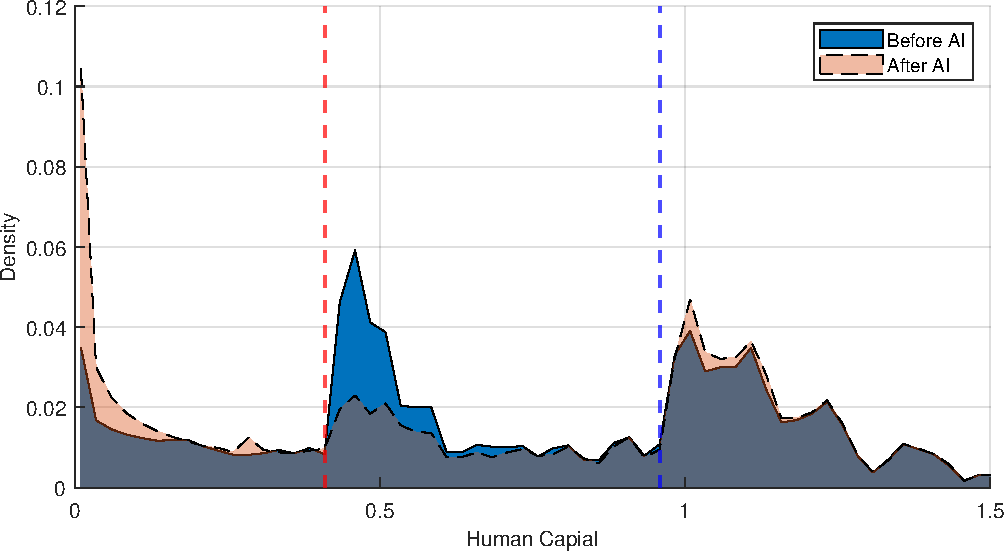
\includegraphics[scale=0.7]{../figure_204040calib/h_dist}
\par\end{center}


\end{frame}

\begin{frame}{Baseline Results {\small\textbf{\textit{\textcolor{brown}{~~Job Polarization}}}}}

\begin{center}
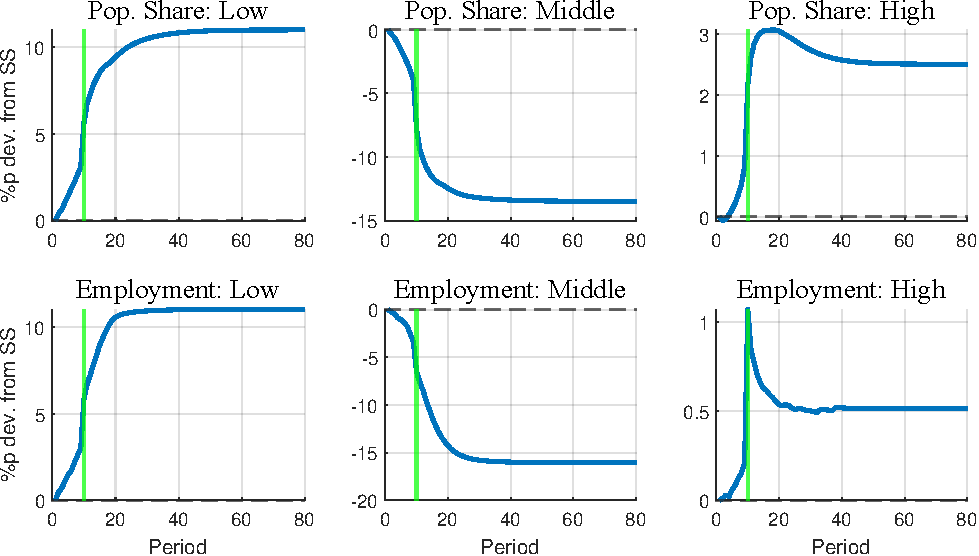
\includegraphics[scale=0.7]{../figure_204040calib/share} 
\par\end{center}

\end{frame}

\begin{frame}{Baseline Results {\small\textbf{\textit{\textcolor{brown}{~~Direct and Indirect
Effects}}}}}
\begin{itemize}
\item Effects of AI reflect two forces:
\begin{itemize}
\item \textbf{Direct effect: }AI changes sectoral productivity, shifting
earnings, labor supply, savings, and aggregate output.
\item \textbf{Indirect effect:} Households respond with human capital adjustment and reallocate across sectors, further affecting productivity
and inequality.

\medskip{}

\end{itemize}
\item To decompose the effect, \textcolor{blue}{we compare the benchmark
model to a Without-HC model}
\begin{itemize}
\item The Without-HC model captures AI's direct effects
\item Gap between benchmark and Without-HC models captures indirect effects. 

\end{itemize}
\end{itemize}
\end{frame}

\begin{frame}{Baseline Results {\small\textbf{\textit{\textcolor{brown}{~~Aggregate Effects}}}}}

\begin{center}
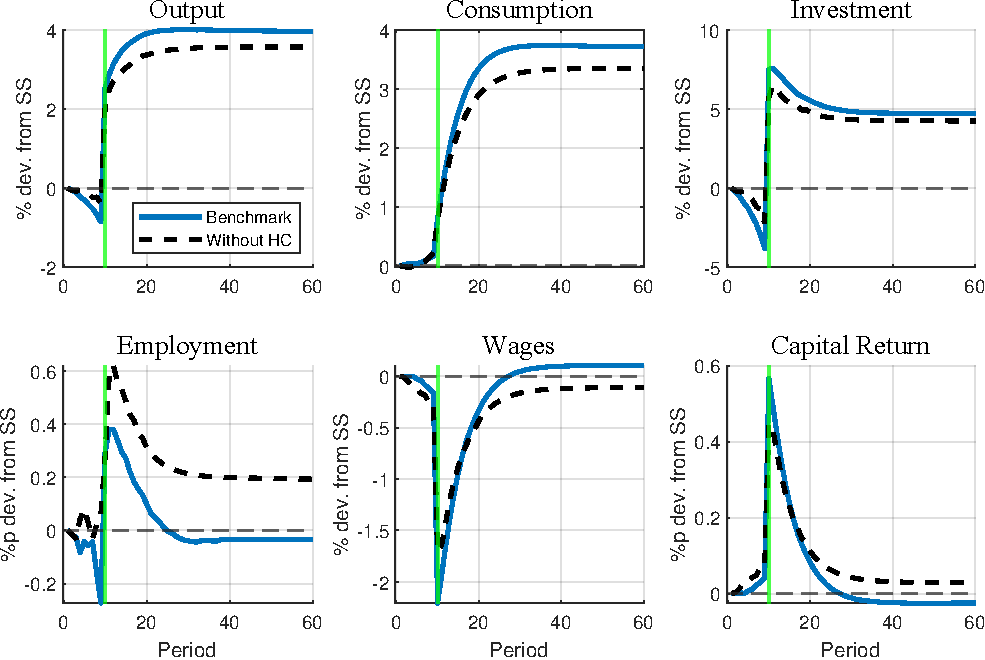
\includegraphics[scale=0.7]{../figure_204040calib/nohc_agg}
\par\end{center}

\end{frame}

\begin{frame}{Baseline Results {\small\textbf{\textit{\textcolor{brown}{~~Distributional
Outcomes}}}}}

\begin{center}
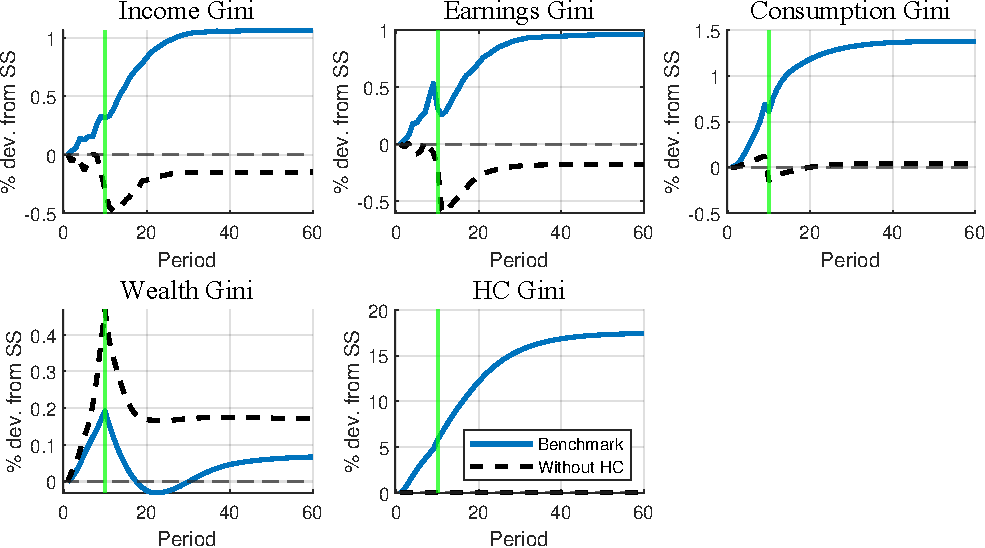
\includegraphics[scale=0.7]{../figure_204040calib/nohc_gini}
\par\end{center}

\end{frame}

\begin{frame}{Baseline Results {\small\textbf{\textit{\textcolor{brown}{~~Wealth Inequality}}}}}

\begin{center}
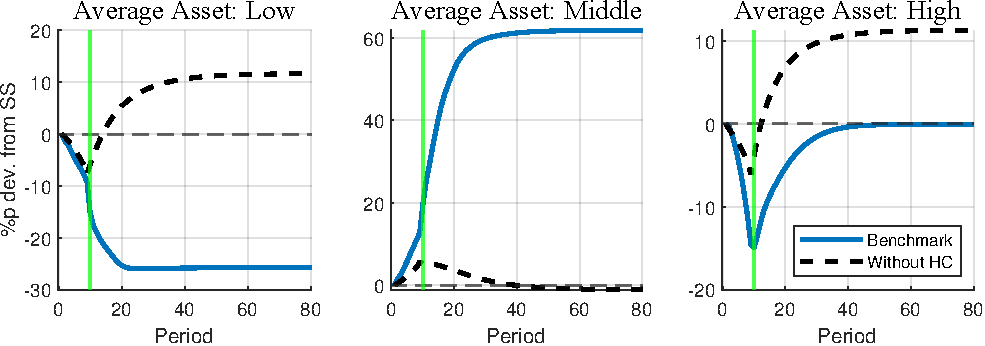
\includegraphics[scale=0.7]{../figure_204040calib/nohc_asset}
\par\end{center}

\medskip{}

\begin{itemize}
\item AI\textquoteright s direct effect: AI affects household saving only
through income effects.
\item Indirect effect from HC: composition channel + \textbf{\textcolor{red}{saving-crowding-in
channel}}
\end{itemize}
\end{frame}

\section{AI+ Results}

\begin{frame}{AI+ Results {\small\textbf{\textit{\textcolor{brown}{~~High Sector}}}}}

\begin{center}
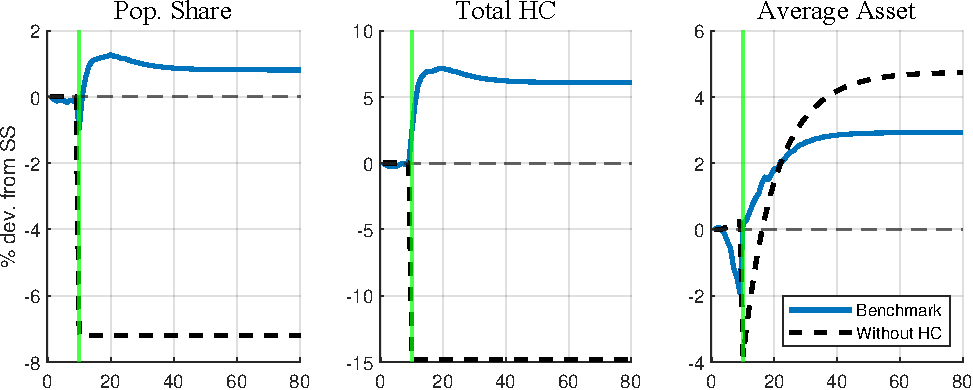
\includegraphics[scale=0.7]{../figure_204040calib/nohc_high_plus}
\par\end{center}

\medskip{}

\begin{itemize}
\item Workers near the new threshold increase
HC investment to stay in the high sector. 
\item They are high-income households so HC investment crowds in their saving.
\end{itemize}
\end{frame}

\begin{frame}{AI+ Results {\small\textbf{\textit{\textcolor{brown}{~~Aggregate
Effects}}}}}

\begin{center}
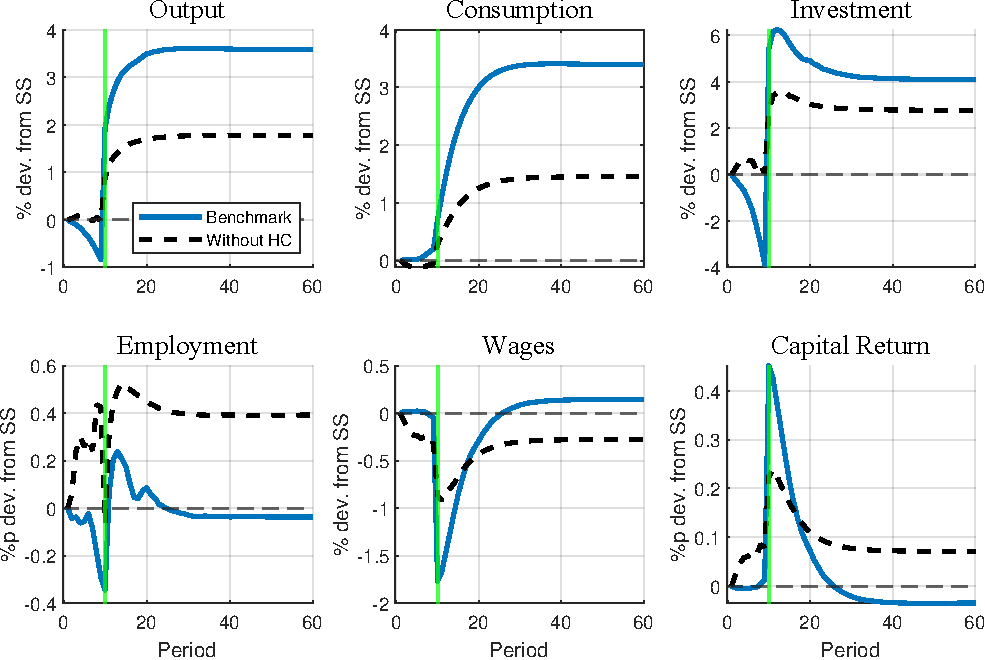
\includegraphics[scale=0.7]{../figure_204040calib/nohc_agg_plus}
\par\end{center}

\end{frame}

\begin{frame}{AI+ Results {\small\textbf{\textit{\textcolor{brown}{~~Distributional
Outcomes}}}}}

\begin{center}
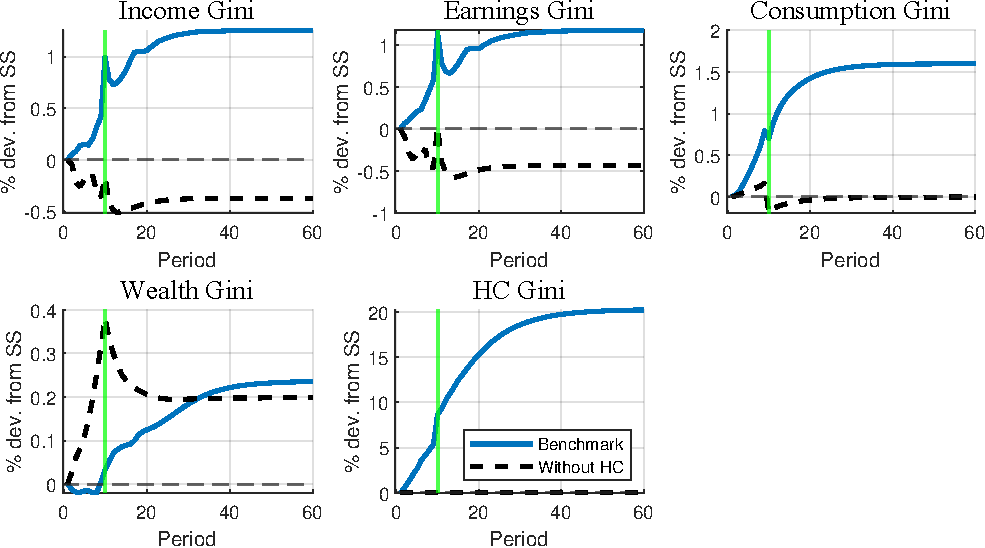
\includegraphics[scale=0.7]{../figure_204040calib/nohc_gini_plus}
\par\end{center}

\end{frame}


\section{Conclusion}
\begin{frame}{Conclusion}

\begin{itemize}
\item \textcolor{black}{This paper analyzes how AI-driven technological
change influences human capital investment and, in turn, affects aggregate
outcomes and economic inequality.}
\item \textcolor{black}{We build an incomplete markets model with endogenous
human capital investment, sectoral structure, transition dynamics,
and general equilibrium feedback.}
\end{itemize}
\bigskip{}

\begin{itemize}
\item \textcolor{black}{AI's effects not only depend on its direct productivity effects, but also }

\item[-] \textcolor{black}{on households' human capital responses; }
\item[-] \textcolor{black}{on human capital's interaction with labor supply 
and precautionary saving.}

\end{itemize}
\end{frame}

\appendix

\begin{frame}{GE effects {\small\textbf{\textit{\textcolor{brown}{~~Aggregate
  Effects}}}}}

  
  \begin{center}
    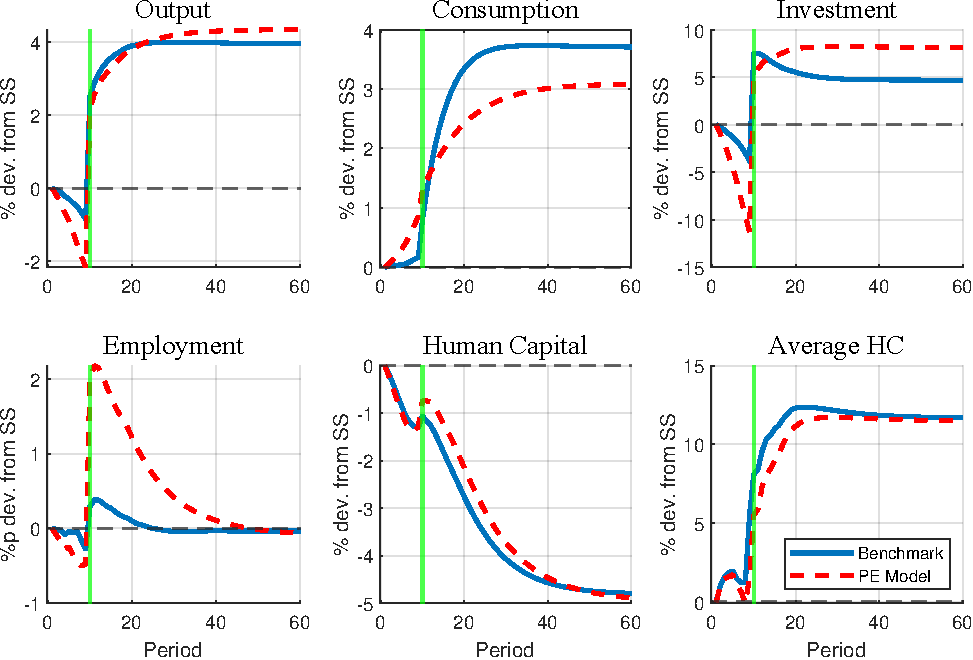
\includegraphics[scale=0.65]{../figure_204040calib/pe_agg.pdf}
  \end{center}


\end{frame}

\begin{frame}{GE effects {\small\textbf{\textit{\textcolor{brown}{~~Distributional
  Effects}}}}}

  \begin{center}
    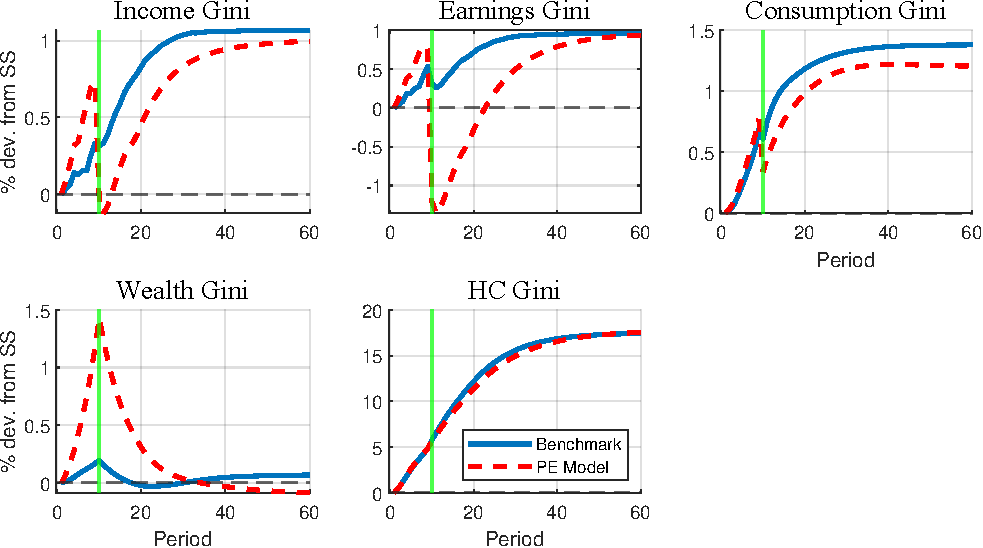
\includegraphics[scale=0.65]{../figure_204040calib/pe_gini.pdf}
  \end{center}
\end{frame}

\end{document}
